\documentclass[border=4pt]{standalone}
\usepackage{tikz}
\usetikzlibrary{arrows.meta}

\newcommand{\smallmap}[2]{%
  \begin{scope}[shift={#1}]
    \draw (0,0) grid (4,2);
    \foreach \x/\lab in {0/00,1/01,2/11,3/10}
      \node[font=\scriptsize] at ({\x+0.5},2.18) {\texttt{\lab}};
    \node[font=\scriptsize] at (-0.25,1.5) {0};
    \node[font=\scriptsize] at (-0.25,0.5) {1};
    \node[font=\scriptsize] at (-0.55,1.0) {$A$};
    #2
  \end{scope}}

\begin{document}
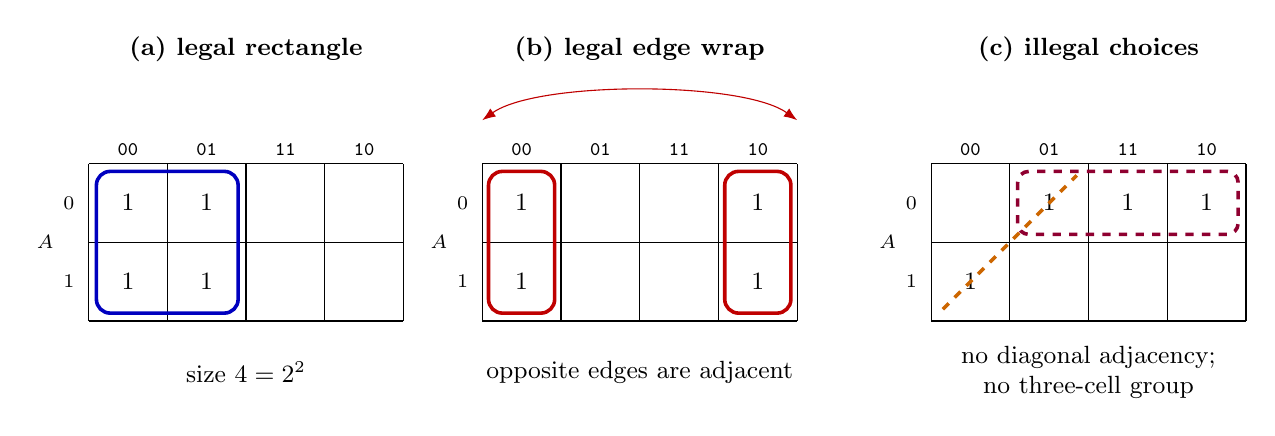
\begin{tikzpicture}[font=\small, >=Latex]
  \node[font=\small\bfseries] at (2,3.45) {(a) legal rectangle};
  \smallmap{(0,0)}{
    \foreach \x/\y in {0/0,1/0,0/1,1/1}
      \node at ({\x+0.5},{\y+0.5}) {1};
    \draw[blue!75!black,line width=1.3pt,rounded corners=5pt]
      (0.1,0.1) rectangle (1.9,1.9);
  }
  \node at (2,-0.65) {size $4=2^2$};

  \node[font=\small\bfseries] at (7,3.45) {(b) legal edge wrap};
  \smallmap{(5,0)}{
    \foreach \x/\y in {0/0,3/0,0/1,3/1}
      \node at ({\x+0.5},{\y+0.5}) {1};
    \draw[red!75!black,line width=1.3pt,rounded corners=5pt]
      (0.08,0.1) rectangle (0.92,1.9);
    \draw[red!75!black,line width=1.3pt,rounded corners=5pt]
      (3.08,0.1) rectangle (3.92,1.9);
    \draw[red!75!black,<->] (0.0,2.55)
      .. controls (0.7,3.05) and (3.3,3.05) .. (4.0,2.55);
  }
  \node at (7,-0.65) {opposite edges are adjacent};

  \node[font=\small\bfseries] at (12.7,3.45) {(c) illegal choices};
  \smallmap{(10.7,0)}{
    \foreach \x/\y in {0/0,1/1,2/1,3/1}
      \node at ({\x+0.5},{\y+0.5}) {1};
    \draw[orange!80!black,line width=1.3pt,dashed]
      (0.15,0.15) -- (1.85,1.85);
    \draw[purple!75!black,line width=1.3pt,dashed,rounded corners=4pt]
      (1.1,1.1) rectangle (3.9,1.9);
  }
  \node[align=center] at (12.7,-0.65)
    {no diagonal adjacency;\\no three-cell group};
\end{tikzpicture}
\end{document}
